%\begin{figure}[htb]
%\centering
%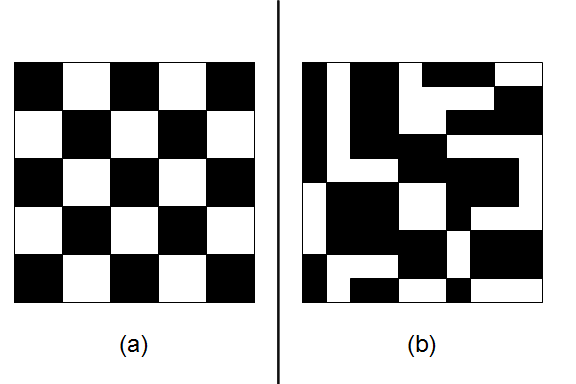
\includegraphics[width=\linewidth]{./graphics/checkers}
%\caption{Monte Carlo Checkerboard Example}
%\label{checker}
%\end{figure}

\subsection{Literature Review}
% present a history of efforts that lead to the DMP as I received it
 **TODO an introductor paragraph or paragraphs, flesh out this section, add more lits?

Three major developments stand as guideposts to the development of the discrete maximum principle as it existed prior to the work described in this thesis.  The first is the acknowledgment made by Fleck and Cummings themselves.  The next milestone came roughly 15 years later when Larsen and Mercier developed the \gls{cmp}.  Finally, another decade and a half later, Wollaber, Larsen, and Densmore brought forth the discrete maximum principle.

\subsubsection{Radiative Heat Transfer Equations}
Before considering the implicit Monte Carlo equations, we first build the concepts leading up to the radiative heat transport equations.

First, we consider the transport of a photon around background material.  We consider the seven dimensions that uniquely describe the photon:
\begin{align}
\mathbf{r} &= \mbox{location in space (3 variables, i.e., $x y z$)},\\
\mathbf{\Omega} &= \mbox{velocity direction (2 variables, i.e., $\theta \phi$)},\\
\nu &= \mbox{frequency (corresponding to photon energy), and}\\
t &= \mbox{time}.
\end{align}

Rather than consider single photons, however, we find it mathematically profitable to consider the photon intensity, $I$, in a particular cross-sectional area.  That is, $I(\mathbf{r}, \mathbf{\Omega}, \nu, t)$, assuming standard metric units, describes the number of photons passing through a centimeter-by-centimeter area in one second having a specific energy and velocity.  This gives the photon intensity units of photons per centimeters-squared-seconds.  Another way to think of this specific intensity $I$ is as an energy density function, meaning that integrating $I$ over space will yield the energy in the radiation within that space \ref{wol_thesis}.  $I$ is given mathematically as
\begin{equation}
I=ch\nu n(\mathbf{r},\mathbf{\Omega},\nu,t),
\end{equation}
where
\begin{align}
n(\mathbf{r},\mathbf{\Omega},\nu,t)dVd\Omega d\nu &= \mbox{mean photons in $dVd\Omega d\nu$ about ($\mathbf{r},\mathbf{\Omega},\nu$) at time $t$,}\\
h&=\mbox{Planck's constant}=6.626\times10^{-35}\mbox{ jk-sh},\\
c&=\mbox{speed of light}=299.793458 \mbox{ cm/sh}.
\end{align}
Above we've made use of the units ``jerk'' (jk, 10$^9$ Joules) and ``shake'' (sh, 10$^{-8}$ seconds).

To completely consider the actions of this photon, we must consider how it can transport from one differential seven-dimension space to another.  It can transport through space by simply moving (or ``streaming'') from one three-dimensional location to another.  It can transport through solid angle by changing its velocity direction (without changing position, necessarily).  The photon can transport through frequency-space by either depositing or absorbing energy, and, lastly, it can transport through time by the simple progression of time from one event to another.

Unfortunately, a single equation with all the sinks and sources discussed above is insufficient to describe the physical system surrounding radiative heat transfer.  The absorption and emission of photons in the background material is largely dependent on temperature.  It is typical to assume the background material and the photons traveling through it (also known as the \emph{radiation field}) are in \gls{lte}.  At its root, this means the material emits photons in a Planckian spectrum and the material's energy can be described by a single temperature \cite{wol_thesis}.  This introduces the second unknown to our problem, the material temperature $T_K(\mathbf{r},t)$ at a particular location and time.  It is likewise typical to express this temperature in units of kilo-electron-volts by multiplying the temperature in Kelvin by Boltzmann's constant.  That is,
\begin{equation}
T(\mathbf{r},t)=kT_K(\mathbf{r},t).
\end{equation}
\indent For a more in-depth discussion of sources and sinks in the radiation field and material, see \cite{pomraming} and TODO 33,34 in Wollaber thesis.  Assuming a one-dimensional system for now, $\mathbf{r}$ becomes $x$ and $\mathbf{\Omega}$ can be uniquely described by $\mu=\cos\theta$ with $\theta$ measured from the positive $x$-axis, we end up with the following coupled system:
\begin{align}\label{eqn_basic_rad}
\frac{1}{c}\frac{\partial I}{\partial t}(x,\mu,\nu,t) + \frac{\partial I}{\partial x}(x,\mu,\nu,t) +
        \sigma_a(x,\nu&,t)I(x,\mu,\nu,t) \nonumber\\
    &=2\pi\sigma_a(x,\mu,t)B(\nu,T) + \frac{Q}{2}(x,\nu,t),
\end{align}
\begin{equation}\label{eqn_basic_mat}
c_v(x,T)\frac{\partial T}{\partial t}(x,t)=
        \int_0^\infty\int_{-1}^1\sigma_a(x,\nu',T)I(x,\mu',\nu',t)
            -2\pi\sigma_a(x,\nu',T)B(\nu',T)d\mu'd\nu',
\end{equation}
for $0\leq x\leq X,-1\leq\mu\leq1,0\leq\nu,$ and $0<t$.  Here, we've introduced
\begin{align}
B(\nu,T)&=\frac{2h\nu^3}{c^2\big[\exp(h\nu/T)-1\big]},\mbox{Planck's radiation function},\\
Q(x,\nu,t)&=\mbox{unspecified photon source},\\
c_v(x,T)&=\mbox{specific heat of the background material},\\
\sigma_a(x,\nu,T)&=\mbox{absorption opacity}.
\end{align}
For the individual familiar with neutronics, the opacity $\sigma$ is analogous to the macroscopic cross section of a material.  Essentially, it describes the probability of a photon being absorbed in the material per unit distance it travels.

In Eqns. \ref{eqn_basic_rad} and \ref{eqn_basic_mat}, the specific intensity $I$ and material temperature $T$ are typically unknown, and everything else is typically given.  Two other useful terms in the development of radiative heat transfer are the material and radiation energy densities, $U_m$ and $U_r$ respectively.  They are given by
\begin{align}\label{eqn_E_density_basic}
\frac{\partial U_m}{\partial T}(x,t)&=c_v(x,t),\\
U_r(x,t)&=aT(x,t)^4,
\end{align}
with $a$ representing the radiation constant,
\begin{equation}
a=\frac{8\pi^5k^4}{15h^3c^3}=0.01372\frac{\mbox{jk}}{\mbox{cm}^3\mbox{keV}^4}.
\end{equation}
It is from this point that Fleck and Cummings began working when they derived the \gls{imc} equations.

\subsubsection{Fleck and Cummings}
 **TODO a sketch of IMC as developed by Fleck and Cummings\\ %%%%%%%
The concerns associated with boundedness of the \gls{imc} equations date back to the first unveiling of the equations themselves.  In their flagship publication describing \gls{imc}, Fleck and Cummings proceeded to demonstrate the viability of their new linearization of the difficult radiative heat transfer equations.  In particular, they looked at a specific Marshak problem with a temporal step size given by $ct=6$ cm, which corresponds to $\Delta_t=TODO$, and a spatial step size of TODO cm.  While smaller time steps resulted in expected behavior, the $ct=6$ cm curve resulted in a strange overheating at the problem boundary nearest the heat source.  Fleck and Cummings acknowledged this, and warned the user to be aware of the problem.


\subsubsection{Larsen and Mercier}
In an effort to direct users to more reliable results when running \gls{imc} problems, Larsen and Mercier understood to derive a maximum principle restriction for time step size.  The intent was to produce a restricting time step size to guarantee physical results, regardless of the spatial step size.
\\ **TODO derivation of continuous maximum principle
Unfortunately, for typical problems, this continuous maximum principle was extremely restrictive in time step, to the point of being impractical for many problems.  Additionally, Larsen and Mercier acknowledge that, for a particular choice of spatial step, physical results were obtained with a time step much larger than the continuous maximum limit suggested possible.  Larsen and Mercier identified two time steps for that spatial step, one of which produced overheating, the other which stayed bounded.  A good maximum principle of necessity would divide these two points.
\\ **TODO add conclusions of Larsen and Mercier papepr


\subsubsection{Wollaber, Larsen, and Densmore}
Finally, in 2011, Los Alamos National Laboratory researchers Wollaber, Larsen, and  Densmore attempted to derive a maximum principle limit for time step that would consider not only temporal discretization as in the continuous maximum principle, but also spatial discretization.
\\ **TODO derivation of discrete max principle
As hoped for, this discrete maximum principle resulted in a limit of temporal and spatial step size that much more closely matches experimental results, including dividing the two points tested by Larsen and Mercier.  While the match was not perfect, it was somewhat conservative, meaning if the user chose a time/space step pair that met the requirements of this discrete maximum principle, it would still be guaranteed not to produce unphysical results in the simulation because of overheating.  While this discrete maximum principle yielded an exciting advancement, it was applied semi-analytically in one dimension making several token assumptions, including equilibrium initial conditions between the background material and radiation field.  Additionally, the only problem run was the Marshak wave problem, where one source of ``hot'' photons are a source on the boundary of a cold material.  This provided a source only on a single side of each cell, simplifying the estimate of energy deposited in a single cell.
\\ **TODO working here

\subsubsection{Summary}
Figure \ref{fig_old_dmps} shows the relationship between the continuous maximum principle, the discrete maximum principle, and experimental results.  The experimental results were obtained using Los Alamos National Laboratory's \texttt{milagro} Monte Carlo \gls{imc} solver.  To find the first maximum principle violation, for each successive time step a logarithmic series of spatial steps were used until the first run that produced a maximum principle violation.  The dash-dot vertical line designates the continuous maximum principle time step limit, while the black dashed line shows the discrete maximum principle limits and the solid blue line is the experimental results.  The discrete maximum principle of Wollaber, Larsen, and Densmore is clearly a huge step in the right direction, and serves as the starting ground for this work.
\\ **TODO add figure of results